\documentclass[aps,pre,reprint,superscriptaddress,amsmath,amssymb,nofootinbib]{revtex4-1}
\usepackage{graphicx}
\usepackage{dcolumn}
\usepackage{bm}
\usepackage{hyperref}
\usepackage{natbib}
\renewcommand{\thefootnote}{\fnsymbol{footnote}}
\DeclareGraphicsExtensions{.pdf}

\begin{document}

\title{Spatially embedded growing small-world networks}
\author{Ari Zitin}
\affiliation{Institute for Research in Electronics and Applied Physics, University of Maryland, College Park, Maryland 20742, USA}
\author{Alex Gorowara}
\affiliation{Institute for Research in Electronics and Applied Physics, University of Maryland, College Park, Maryland 20742, USA}
\author{Shane Squires}
\affiliation{Institute for Research in Electronics and Applied Physics, University of Maryland, College Park, Maryland 20742, USA}
\affiliation{Department of Physics, University of Maryland, College Park, Maryland 20742, USA}
\author{Mark Herrera}
\affiliation{Institute for Research in Electronics and Applied Physics, University of Maryland, College Park, Maryland 20742, USA}
\affiliation{Department of Physics, University of Maryland, College Park, Maryland 20742, USA}
\author{Tom Antonsen}
\affiliation{Institute for Research in Electronics and Applied Physics, University of Maryland, College Park, Maryland 20742, USA}
\affiliation{Department of Electrical and Computer Engineering, University of Maryland, College Park, Maryland 20742, USA}
\affiliation{Department of Physics, University of Maryland, College Park, Maryland 20742, USA}
\author{Michelle Girvan}
\affiliation{Institute for Research in Electronics and Applied Physics, University of Maryland, College Park, Maryland 20742, USA}
\affiliation{Institute for Physical Science and Technology, University of Maryland, College Park, Maryland 20742, USA}
\affiliation{Department of Physics, University of Maryland, College Park, Maryland 20742, USA}
\author{Edward Ott}
\affiliation{Institute for Research in Electronics and Applied Physics, University of Maryland, College Park, Maryland 20742, USA}
\affiliation{Department of Electrical and Computer Engineering, University of Maryland, College Park, Maryland 20742, USA}
\affiliation{Department of Physics, University of Maryland, College Park, Maryland 20742, USA}

\date{\today}

\begin{abstract}
Networks in nature are often formed within a spatial substrate in a dynamical manner, gaining links and nodes as they develop over time. 
Motivated by biological considerations, we propose a class of growing network models and investigate the relationship between the resulting statistical network properties and the space in which the networks are embedded. 
In particular, we consider models in which nodes are placed one by one in random locations in space, with each such placement followed by configuration relaxation toward uniform node density, and connection of the new node with spatially nearby nodes. 
We characterize the spatial and topological properties of these networks and show how spatial embedding supports the emergence of small-world networks.
\end{abstract}

\pacs{05.45.-a, 05.65.+b, 89.75.-k, 89.75.Fb ,89.75.Hc} %Nonlinear dynamics and chaos, Self-organized systems, Complex Systems, Structures and organization in complex systems, Networks and genealogical trees

\maketitle

\section{INTRODUCTION}
%in the introduction don't forget to present definitions we use, in particular be clear what we mean by small world property
%mention how our generalizations were chosen for their physical significance rather than the ease with which we can perform comupational and analytic calculations of their properties. 
Haven't written the introduction yet but we intend to cite:
\cite{wsnat}, \cite{ozik2004}, \cite{przuljgeo}, \cite{hermannspace}, \cite{bullockspatial}, \cite{guan1D}, \cite{zhang2006}, \cite{zhang2007}, \cite{newmanreview}  as prior work on the subject.
We also intend to cite:
\cite{neuronembedding}, \cite{plenzcascade}, \cite{fruitfly}, \cite{barthelemy}, \cite{vazquez2002} as examples of applications of spatial network models.

\section{THE CIRCLE MODEL}
In Ref. \cite{ozik2004} the authors presented a model, henceforth referred to as the Circle Mode, which considers a network which initially has $m+1$ uniformly separated, all-to-all connected nodes on the circumference of a circle. 
At each discrete time step the network is grown according to the following rules: 
(1) a new node is placed at a randomly selected point on the circumference of the circle;
(2) the new node is linked to its $m$ nearest neighbors;
(3) preserving node positional ordering, the nodes are repositioned to make the nearest-neighbor distance uniform;
(4) steps (1-3) are repeated until the network has $N$ nodes.
Since the network is incremented in size by one node each timestep, the network size $N$ can also be used as the system time parameter.  
It has been shown \cite{ozik2004} that this growth model leads to a small-world network with an exponentially decaying degree distribution. 
The original goal of the Circle Model was to explore the effect that geographic attachment locality has on the growth of networks.
In this paper, we extend this analysis by considering networks growing by geographic attachment preference in more general Euclidean spaces. 

We defined a network growth procedure to yield the small-world property if, as $N \to \infty$,
(i) the average degree $\langle k \rangle$ of a node approaches a non-zero value,
(ii) the graph characteristic path length (defined as the average value of the smallest number of links joining node pairs) does now grow with $N$ faster than $\log N$, and
(iii) the clustering coefficient (defined below) does not approach zero.
The original Circle Model exhibits these properties.
\begin{itemize}
  \item \textbf{Degree Distribution:} The degree distribution $H(k)$ is the probablility that a randomly selected node has $k$ network connections at time $N$.
For large $N$, the degree distribution of the Circle Model is given by 
\begin{equation}\label{degdist}
H(k) = \frac{1}{m+1}\left(\frac{m}{m+1}\right)^{k-m}
\end{equation}
for $k \geq m$ and $H(k) = 0$ for $k < m$ \cite{ozik2004}.
Since the number of new links added each time a new node is added is $m$, Eq. \ref{degdist} yields the result that, the average node degree $\langle k \rangle$ is $2m$, satisfying the first criterion (i) for the small-world property.
  \item \textbf{Characteristic Path Length:} In the Circle Model, simulation results show the path length scaling, $\ell \sim \log N$ [criterion ii].
This may be explained intuitively by noting that as new nodes are added they push apart the older connected nodes, lengthening the distance traversed by older edges. 
These older nodes can then have geographically long links, thus dramatically decreasing the shortest graph path length between any given pair of nodes.
  \item \textbf{Clustering Coefficient:} For the Circle Model it was shown  that the clustering coefficient approaches a constant, positive, $m$-dependent value as $N \to \infty$ [criterion (iii)]. 
The clustering coefficient of a network is the fraction of connected triples which are also triangles.
This measures whether two nodes which are both connected to a third node are likely to be connected to one another. \footnote{In \cite{ozik2004} an alternate definition of clustering was used, specifically, the average of the local clustering $C_i$ of each node, $C_i = q_i/[\frac{1}{2} k_i (k_i-1)]$ where $q_i$ is the number of links between the $k_i$ neighbors of node $i$.}
\end{itemize}
The Circle Model, being fundamentally limited by the supposed one-dimensional and spatial periodicity of the underlying space (a circle), naturally raises the question of whther similar properties apply for other types of underlying spaces, e.g., spaces with higher dimensionality. 
The goal of this paper is to address this question.

\section{The Sphere Problem}
One natural generalization from embedding nodes on the one-dimensional circumference of a circle is to embed them on the two-dimensional surface of a sphere, or in general on the $d$-dimensional surface of a hypersphere.
On a circle it is trivial to arrange $N$ points along the circumference with uniform spacing, but the analogous procedure is less well-defined on higher dimensional surfaces.
One way to generalize the arrangement procedure is to consider nodes to be point charges and to move them to a minimum electrostatic energy equilibrium configuration. 
The problem of finding the equilibrium configuration of point charges on the surface of a sphere dates back to 1904 when J.J. Thomson introduced his model of the atom, and the problem of obtaining such an equilibrium is sometimes referred to as the `Thomson problem' \cite{thomson1904}.

Using the Thomson problem as a guide, we develop one of our generalizations to the Circle Model, which we call the Sphere Model, as follows.
We model the nodes as point charges confined to exist on the surface of a $d$-sphere of unit radius.
Now, at each timestep, we drop a new node onto the sphere at random with uniform probability density per unit area and then add links to connect it to its $m$ nearest neighbors, where here distance is defined as the shortest great circle path along the surface of the sphere between two nodes.
Next we minimize the potential energy of the configuration by a steepest descent procedure, $\frac{d\underline{x}_i}{dt} = -\bigtriangledown_\parallel V$, where $V$ is the potential, $\underline{x}_i$ is the position of node $i$, and $\bigtriangledown_\parallel$ represents the projection of the $d$-dimensional gradient operator onto the surface of the sphere.
Note that, as new nodes are added, this procedure tends to yield a local energy minimum, as opposed to the global minimum, and we view this as being appropriate for the situations of interest to us (e.g., biological network growth processes).
For large $N$, the repulsive interaction ensures that the points are distributed approximately uniformly on the surface of the $d$-sphere.
In this way we reproduce the key features of the Circle Model, but we also introduce a new parameter, the dimension of the space in which the growing network is embedded.
For a $2$-sphere in $3$-space, this is similar to the original Thomson problem presented in \cite{thomson1904}, where $N$ electrons are bound to the surface of a sphere and interact with each other via the $2$ dimensional Couloumb force.
For the case of a $d$-dimensional sphere embedded in $d+1$-dimensional space, we use as our repulsive term the Coulomb force law appropriate to a $d$-dimensional space (namely, force $\sim r^{-(d-1)}$).

As a result of the Couloumb interaction, the minimum energy configuration for these points on the sphere is one where the points are distributed in an approximately uniform manner on the surface of the sphere.
In order to determine if this model produces a small world network we determine the following three properties:
\begin{itemize}
  \item \textbf{Degree Distribution:} The approximately uniform distribution of nodes on the surface of the $d$-sphere leads to an approximately equal probability of nodes having their degree increased by a link to a new node at each timestep.
In accord with this, we fill find that the degree distribution for this new model is identical to the degree distribution for the original Circle Model (for more detail see Sec.~\ref{sec:degreedistribution}).
  \item \textbf{Characteristic Path Length:} For this model we find that the the average shortest path length $\ell$ scales logarithmically with the network size $N$, that is, $\ell \sim \log N$. 
This is a reasonable result because as the network grows in size the older nodes get pushed apart by the repulsive Coulumb force thus leaving bridges across the network that span a significant geographic distance.
These long range links serve to connect disparate regions of highly interconnected nodes, dramatically reducing the shortest path length between any two nodes in the network.
At each timestep only geographically local connections are made, but due to the dynamic nature of the nodes' spatial positions, each timestep can make existing links longer in physical space, thus building bridges across the network.
Furthermore, we find that for a given value of $N$ the shortest path between any two nodes in this case is shorter than that of the corresponding 1D case (the original OHO model).
In fact we find that as we increase the dimension $d$ of the embedding space the shortest path shrinks, although it keeps the logarithmic scaling with $N$ that we require for small-worlds.
One possible explanation for this feature is that the surface of a higher dimensional sphere provides more freedom for nodes to move around each other, thus increasing the chance that a shortcut is created.
In the original OHO model each node, like a boson in a Tonks-Girardeau gas, is forever locked between its two original spatial neighbors, and thus long range links can only be created if new nodes are placed between the two neighbors.
Here the repulsive Couloumb force between electrons allows them to rearrange thier relative positions by moving in $d$ dimensions in order to minimize the potential energy of the configuration.
Thus two originally adjacent nodes can be moved apart around other nodes, forming long range links; of course placing new nodes between them will also create bridges, but these effects combine to produce shorter path length in the higher dimensional cases.
  \item \textbf{Clustering Coefficient:} This section has not yet been written since we're waiting on the results of the force law investigation to come to a conclusion about clustering. 
%I'm going to leave this section blank until we have results and figures for this since that should determine what we write.
\end{itemize}
Thus we find that that the model of a network growing on the surface of a $d$-sphere with geographic attachment preference leads to the emergence of the small-world property.

\section{THE PLUM PUDDING MODEL}
The Sphere Model described above has the feature that the geographical embedding region does not have an edge.
Thus we have also tested another model with different topology.
We call this second model the Plum Pudding Model.

We again model our nodes as a collection of negative point charges in $d$-dimensions.
The growth procedure is similar to the previous models; we place new nodes randomly in our volume and connect them to their $m$ nearest neighbors, where here we define nearest to be the Euclidean distance between the nodes.
Now, however, we regard the nodes as free to move in a unit radius, $d$-dimensional sphere containing a uniform background positive charge density such that the total background charge in the sphere is equal and opposite to that of the $N$ network nodes.
Similar to our previous mode, after adding a node with uniform probability density within the unit $d$-dimensional sphere, we relax the configuration to a local energy minimum via the process $\frac{d\underline{x}_i}{dt} = -\bigtriangledown V$, where $\bigtriangledown$ is the $d$-dimensional gradient operator.
The repulsive potential between nodes ensures that they are spaced approximately equidistantly for large $N$ in a minimum potential configuration, while the cloud of positive charge ensures that the nodes remain in the sphere.

Due to the nature of Gauss's Law for any dimension $d$ the `force` of attraction between a node and the center of the background constant-density positive charge cloud is proportional to the value of the radial coordinate of the node.
This means that we can visualize this model as a collection of classical electrons all connected to the origin by springs (a harmonic potential) and interacting with each other via the dimensionally appropriate Couloumb force.  

We now consider the one-dimensional Plum Pudding Model on a line segment and compare it to the original Circle Model.
For the electrostatic problem on a one-dimensional line segment, we regard the node particles as charge sheets, which, through Gauss's law, leads to a constant repulsive force between electron pairs, thus the equilibrium for both the analogouse $1$-d sphere (i.e. Circle) and Plum Pudding Models yields equally spaced nodes. 
On the circle every node borders two internode intervals, while on the line segment, this is so for $(N-2)$ interior nodes with only the two boundary nodes bordering just one internode interval.
Thus as $N \to \infty$, the one-dimensional Plum Pudding Model is expected to yield results that are identical to those of the Circle Model.
Two fundamental properties of our one-dimensional models are that, when a new node is added, relaxation to equilibrium preserves the relative spatial ordering of nodes, and the equilibrium has uniform internodal spacing.
In contrast, for $d \geq 2$ the concept of linear ordering is absent.
In addition, for our $d \geq 2$ sphere and plum pudding topologies, exact, global regular-lattice positioning is not possible.
E.g., for large $N$ on a $2$-d sphere, it is known that, although equilibrium positioning through much of the area of the sphere is locally approximately a regular triangular lattice, the sphere's surface curvature leads to point and line defects in the triangular lattice pattern \cite{nelson}.
Thus a natural question is whther the $d = 1$ cases might have special properties that deviate from those for $d \geq 2$.

\section{INVARIANT PROPERTIES}
Several important network features can be found analytically and do not depend on dimension or on the choice of the plum pudding or Sphere Model.
A key observation in each of the following derivations is that the probability that each newly added node will form an edge to any particular existing node is $m/N$ for all nodes.
This is because existing nodes are distributed approximately uniformly, and new nodes are placed randomly according to a uniform probability distribution.

\subsection{Degree Distribution}
\label{sub:degreedistribution}
Here we show that for each considered model, we produce the same master equation governing the evolution of the degree distribution (in particular the master equation for the degree distribution in \cite{ozik2004}).  
This master equation is not specific to the spatial structure of the network and appears, in various forms, in other network models, such as the Deterministic Uniform Random Tree of Ref. \cite{zhang2008topologies}.

We define $\hat{G}(k,N)$ to be the number of nodes with degree $k$ when we are at time $N$ (i.e. when the system has $N$ nodes).
When a node is added to the network it is initially connected to its $m$ nearest neighbors, so initially (upon creation) $k = m$ for each node, meaning that $\hat{G}(k,N) = 0 \text{ for } k < m$.
Since each existing node is equally likely to be chosen to be connected to the new node, there is a $\frac{m}{N}$ probability that any given node with have its degree incremented by 1.
Averaging $\hat{G}(k,N)$ over all possible random node placements we get a master equation for the time evolution of $G(k,N)$, the average of $\hat{G}(k,N)$ over all possible randomly grown networks;
\begin{equation}
G(k,N+1) = G(k,N) - \frac{m}{N}G(k,N) + \frac{m}{N}G(k-1,N) + \delta_{km},
\end{equation}
\noindent where $\delta_{km}$ is the Kronecker delta function.
The first term on the right is the expected number of nodes with degree $k$ at time $N$.
The second term is the expected number of nodes with degree $k$ at time $N$ that get promoted to degree $k+1$.
The third term is the expected number of nodes with degree $k-1$ at time $N$ that get promoted to degree $k$.
The last term on the right is the new node with degree $m$.

It was shown by Ozik et al. \cite{ozik2004} that this master equation leads to an exponentially decaying degree distribution with an asymptotically $N$ invariant form $H(k) = \lim_{N \to +\infty} G(k,N)/N$ given by
\begin{equation}\label{degeq}
H(k) = \frac{1}{m+1}\left(\frac{m}{m+1}\right)^{k-m}.
\end{equation}
\noindent for $k \geq m$ and $H(k) = 0$ for $k < m$.

\begin{figure}
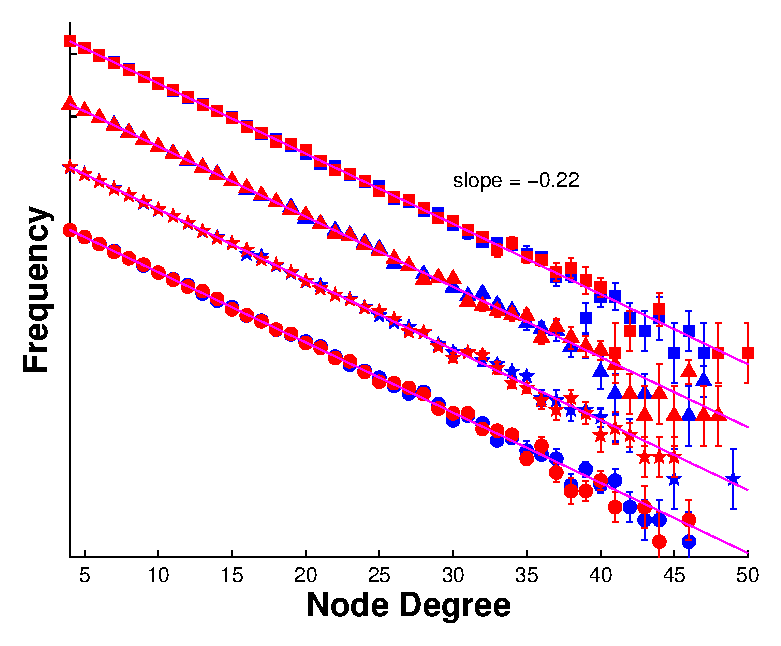
\includegraphics[width=\linewidth]{figures/fig11.pdf}
\caption{\label{degdist}Semilogarithmic graph of the degree distribution for 8 models with $N = 10000$ and $m = 4$ compared to the theory in Eq. \eqref{degeq}; the blue points represent the Sphere Model while the red points represent the Plum Pudding model. The dimensions are represented as follows, 1D - circle; 2D - star; 3D - triangle; 4D - square. Note that an arbitrary linear offset was used to separate data for visualization and thus values on the y-axis are only relative.}
\end{figure}
Interestingly, this exponentially decaying degree distribution comes only from the growth process and the uniform probability of attaching new links to existing nodes.  
As seen in Fig. \ref{degdist}, for $m = 4$, $N = 10^4$, with $d = 1,2,3,4$, Eq. \eqref{degeq} is well-satisfied by numerical simulations of both the Sphere (blue points) and Plum Pudding (red points) Models.

\subsection{Mean Degree as a Function of Node Age}
We seek an expression for the expected degree $k(y,N)$ of a node that has existed for $y$ time steps given that the network size is $N$ ($y < N$).
Each node connects to its $m$ nearest neighbors upon creation, and the probability of incrementing the degree of the node is $m/N$, when the size of the network is $N$.
Thus we obtain 
\begin{equation}\label{ageeq}
\begin{split}
k(y,N)& = m + m\sum_{n=N-y+1}^{N} \frac{1}{n}\\
      & \approx m + m \log \frac{N}{N-y} + \mathcal O\left(\frac{1}{N^2}\right)
\end{split}
\end{equation}
 
Once again, since this derivation uses only the assumption that each node has an equal chance each timestep to have its degree incremented, the result holds for both of the models discussed here.
This represents a specific example of the fact that in dynamically growing networks, older nodes are preferentially connected to one another as discussed in \cite{reallyrandom}.
\begin{figure}
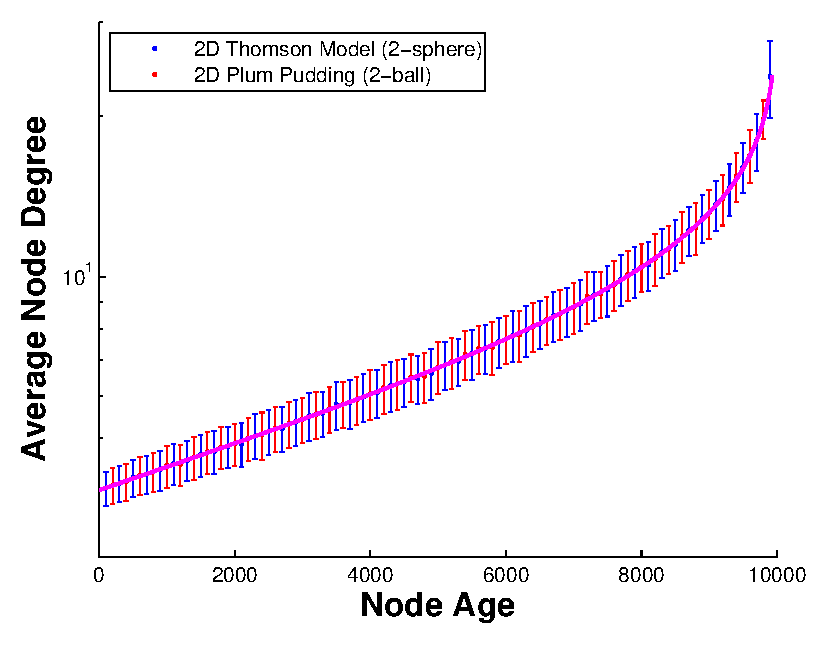
\includegraphics[width=\linewidth]{figures/fig12.pdf}
\caption{\label{degage}Semilogarithmic graph of the mean degree vs the node age for two of the explored models with $N = 10000$ and $m = 4$. The magenta line is the theory in Eq. \eqref{ageeq} and the error bars are the standard deviation of the average over 10 simulated networks}
\end{figure}
Numerical simulations of the mean degree as a function of node age, Fig. \ref{degage}, demonstrate that Eq. \eqref{ageeq} is satisfied for both the Sphere (blue points) and Plum Pudding (red points) models.
Results are only presented for the $2$-dimensional case for simplicity, but the Eq. \eqref{ageeq} has no dependence on the embedding space, and thus holds for other dimensions as well.

\subsection{Betweenness-Degree Relationship}	%this section may not even be necessary...
Betweenness centrality is a common measure of the importance of a node to the propagation of information through a network.
Formally it is the fraction of shortest paths between all node pairs which pass through a given node.
In general we would expect that the nodes with the greatest degree tend to have the highest betweenness.
The existence and subsequent high betweenness of high degree nodes is directly related to the small-world property.
%present figure of betweenness-vs-degree for some of the models and discuss results

\section{Limitations of the Model}
\textbf{****** I'm not sure that we will need to include this section, the key points could be dispersed through the paper instead******}
As with any simulation, our models were limited in the degree to which they could accurately represent a ``real" scenario while still remaining practically computable.  
In this section, we discuss the necessary shortcomings we have identified in our model, and the effects we believe them to have had on our results.  
We first note that the results we have obtained, while certainly biased in one way or another, still appear to accurately represent a genuine trend in the phenomena we investigated, and that the various biases come together to produce what is best characterized as random error, rather than a fundamental flaw.
%the above sentence needs to be clarified, noise is not a good term for what we're talking about.

\subsection{Tolerance of Non-Equilibrium Configurations}
As noted above, we used a gradient-descent method to enforce the even spacing of nodes.  
In order to ensure that the computation halted, we introduced a ceiling on the number of iterations of gradient-descent steps, so that a persistent disequilibrium could not delay the model indefinitely.  
We also introduced a tolerance parameter related to the average inter-node spacing (a function of $N$) such that if all nodes were displaced by less than a certain distance in a single timestep, the gradient-descent algorithm could exit early.  
Both of these steps were necessary to ensure that the use of the model was practically feasible given finite computing resources.
%the above discussion isn't particularly relevant to the context of our paper; perhaps it could be relegated to a document summarizing the code?
Varying the tolerance, we found that a higher tolerance (resulting in fewer steps before exiting the algorithm) correspondeds to decreased displacement of nodes, as was expected.  
Similarly, in cases in which the ceiling on the number of steps was too low (that is, low enough to be encountered frequently), there was less movement than in cases in which the ceiling was high.  
Both of these effects were trades between accuracy and speed; a faster computation meant less displacement, corresponding to a higher clustering coefficient, among other measures.
%again I don't think our audience cares about this.

\subsection{Time Step Size}
For the gradient-descent algorithm, as it was not possible to simulate a truly continuous system, the gradients of each node were calculated and applied in discrete timesteps.  
The size of this timestep tended to be inversely proportional to the time to run a model, so larger time steps were preferable to smaller ones.  
However, larger time steps increased the probability of overshooting the equilibrium (an error which would then be remedied in subsequent iterations of or calls to the algorithm), where smaller timesteps would have prevented such movements by recalculating forces more frequently.

Large time steps, therefore, were also a trade between accuracy and speed, though here, a faster computation meant more displacement.  
The effect of this overshoot is to rearrange the relative position of nodes, pulling apart communities of nearby nodes.
This was reflected in a lower clustering coefficient for rather large time steps, an effect which persisted even for large networks.
%In order to make this claim, you will need more evidence as well as an explanation linking movement to clustering

\subsection{Force Laws} %maybe this section can be expanded to it's own section where we justify the choice of force law we used and mention how higher force exponent leads to more numerical problems??
In calculating the gradients for the gradient-descent algorithm, we used a scaling taken from the Coulomb force in an arbitrary number of dimensions: $F \propto \frac{1}{r^{d-1}}$ in a $d$-dimensional space.  
For the $d$-dimensional ball, the ball and the space in which it was embedded were of the same dimension, which as the dimension used there.  
In the case of the $d$-dimensional sphere, however, the dimension of the sphere itself, which was one less than that of the embedding space, was used, which produced results approximately similar to those produced from the $d$-dimensional ball.

However, we found that different force laws produced substantially different arrangements.  %More to follow once we have conclusive data on force/dimension.

\subsection{Error Summary}
Based on informal comparisons to networks using small $N$, we have come to the conclusion that while the error introduced by these factors does affect the properties of the networks, the effects do, to some extent, act against each other.  Increased tolerance results in insufficient movement, while increased timestep size results in extra movement.  With that in mind, and in light of the ``growing" nature of our models, it may be appropriate to slightly change our concept of the model.  Rather than converging to a static state, our models instead experience a substantial excitation upon the addition of a new node, but then return to what is akin to a dynamic equilibrium, the activity of its members no longer organized or large.  We believe this is a better analogy for real growing networks, which are rarely truly static.

\section{CONCLUSION}
%Write the conclusion at the end when we have all of the results and figures and even after we've written the introduction, make sure to keep the conclusion short

\bibliography{grownet}

\end{document}

